\documentclass[aspectratio=169,11pt]{beamer}
\usetheme{default}
\setbeamertemplate{navigation symbols}{}
\setbeamertemplate{footline}{%
  \hfill\insertframenumber/\inserttotalframenumber\hspace*{4pt}\vspace{2pt}%
}
\usepackage{lmodern}
\usepackage[most]{tcolorbox}
\usepackage{listings}
\usepackage{tikz}
\usetikzlibrary{arrows.meta,positioning,shapes.geometric,fit,backgrounds}
\usepackage{booktabs}
\usepackage{hyperref}

\definecolor{lcgreen}{HTML}{2E7D32}
\definecolor{lcblue}{HTML}{1565C0}
\definecolor{lcorange}{HTML}{EF6C00}
\definecolor{lcred}{HTML}{C62828}
\definecolor{codebg}{HTML}{F5F5F5}
\definecolor{docgray}{gray}{0.55}

\newtcolorbox{conceptbox}[1][]{colback=yellow!20,colframe=yellow!60!black,title=#1,fonttitle=\bfseries}
\newtcolorbox{warningbox}[1][]{colback=red!15,colframe=red!60!black,title=#1,fonttitle=\bfseries}
\newtcolorbox{tipbox}[1][]{colback=green!10,colframe=green!50!black,title=#1,fonttitle=\bfseries}
\newtcolorbox{codebox}[1][]{colback=blue!10,colframe=blue!40!black,title=#1,fonttitle=\bfseries}

\lstset{
  basicstyle=\ttfamily\scriptsize,
  backgroundcolor=\color{codebg},
  breaklines=true,
  frame=single,
  rulecolor=\color{blue!40!black},
  keywordstyle=\color{lcblue}\bfseries,
  stringstyle=\color{lcgreen},
  commentstyle=\color{docgray}\itshape,
  language=Python,
  showstringspaces=false,
  tabsize=2,
  xleftmargin=2pt,
  xrightmargin=2pt,
}

\newcommand{\docref}[1]{{\scriptsize\color{docgray}[Docs: #1]}}

\title{LangChain v1.2.x: Tools \& Tool Calling}
\subtitle{Making LLMs interact with the real world}
\author{LangChain Framework}
\date{March 2026}

\begin{document}

% ============================================================================
% SLIDE 1: Title Slide
% ============================================================================
\frame{\titlepage}

% ============================================================================
% SLIDE 2: Agenda
% ============================================================================
\begin{frame}[fragile]{Agenda}
\begin{itemize}
  \item Mental model: Tools as bridges to the real world
  \item Tool definitions: what is a tool?
  \item Creating tools: decorators and explicit schemas
  \item Tool schemas and model binding
  \item Tool calling flow and execution patterns
  \item Advanced: async, validation, MCP integration
  \item Common pitfalls and best practices
  \item Self-check quiz
\end{itemize}
\vfill
\textcolor{docgray}{\small By the end: you'll be able to create, bind, and invoke tools with LLMs}
\end{frame}

% ============================================================================
% SLIDE 3: Mental Model - Tools as Bridges
% ============================================================================
\begin{frame}[fragile]{Mental Model: Tools as Bridges}
\begin{center}
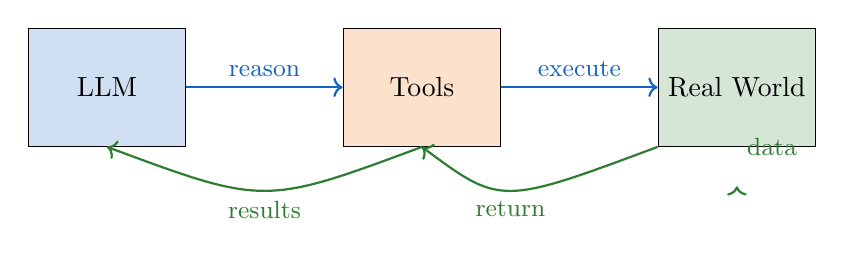
\begin{tikzpicture}[scale=1.0]
  % LLM box
  \node[draw, rectangle, fill=lcblue!20, minimum width=2cm, minimum height=1.5cm]
    (llm) at (0, 0) {LLM};

  % Tools box
  \node[draw, rectangle, fill=lcorange!20, minimum width=2cm, minimum height=1.5cm]
    (tools) at (4, 0) {Tools};

  % Real World box
  \node[draw, rectangle, fill=lcgreen!20, minimum width=2cm, minimum height=1.5cm]
    (world) at (8, 0) {Real World};

  % Arrows
  \draw[->, thick, color=lcblue] (llm.east) -- (tools.west)
    node[midway, above, color=lcblue] {\small reason};
  \draw[->, thick, color=lcblue] (tools.east) -- (world.west)
    node[midway, above, color=lcblue] {\small execute};
  \draw[->, thick, color=lcgreen] (world.south) -- (world.south) + (0, -0.5)
    node[midway, right, color=lcgreen] {\small data};
  \draw[->, thick, color=lcgreen] (world.south west) .. controls (5, -1.5) .. (tools.south)
    node[midway, below, color=lcgreen] {\small return};
  \draw[->, thick, color=lcgreen] (tools.south) .. controls (2, -1.5) .. (llm.south)
    node[midway, below, color=lcgreen] {\small results};
\end{tikzpicture}
\end{center}

Tools are the mechanism for LLMs to \textbf{perceive and act} on the world beyond text completion.

\begin{tipbox}[Key Insight]
Without tools, LLMs can only talk about things. With tools, LLMs can \textit{do} things.
\end{tipbox}
\end{frame}

% ============================================================================
% SLIDE 4: What is a Tool? Definition
% ============================================================================
\begin{frame}[fragile]{What is a Tool? Core Definition}
\begin{conceptbox}[A Tool is...]
\small
A callable interface between an LLM and an external system, defined by:
\begin{itemize}
  \item \textbf{Name}: unique identifier (e.g., \texttt{search\_documents})
  \item \textbf{Description}: human-readable explanation for the LLM
  \item \textbf{Schema}: input type, argument names, types, descriptions
  \item \textbf{Callable}: Python function that executes the tool
  \item \textbf{Return type}: what the tool outputs (typically str or structured)
\end{itemize}
\end{conceptbox}

\begin{codebox}[Example Tool (conceptual)]
\lstinline{Tool(name="get_weather", description="...", schema={...}, func=get_weather_impl)}
\end{codebox}

\textcolor{docgray}{\docref{langchain.tools.tool}}
\end{frame}

% ============================================================================
% SLIDE 5: Tool Invocation Flow
% ============================================================================
\begin{frame}[fragile]{Tool Invocation Flow}
\begin{enumerate}
  \item LLM receives user query + bound tools
  \item LLM \textbf{decides} which tool(s) to call (if any)
  \item LLM returns \texttt{tool\_calls}: list of \{name, args\}
  \item Application \textbf{executes} the tool with args
  \item Application returns \texttt{ToolMessage} with results
  \item Optionally, LLM processes results and calls more tools
\end{enumerate}

\vfill

\begin{tipbox}[Critical Point]
The LLM \textbf{never directly executes} the tool. It decides to call it; you execute it.
\end{tipbox}
\end{frame}

% ============================================================================
% SLIDE 6: The @tool Decorator
% ============================================================================
\begin{frame}[fragile]{The @tool Decorator: Quick Start}
\begin{codebox}[Simplest Way to Create a Tool]
\begin{lstlisting}
from langchain.tools import tool

@tool
def get_weather(city: str) -> str:
    """Get current weather for a city.

    Args:
        city: City name (e.g., 'New York')

    Returns:
        Weather description
    """
    # Simulated weather lookup
    return f"Weather in {city}: Sunny, 72 F"

# Use it
tool_obj = get_weather
print(tool_obj.name)  # "get_weather"
print(tool_obj.description)  # docstring used as description
\end{lstlisting}
\end{codebox}

\textcolor{docgray}{\docref{langchain.tools.tool}}
\end{frame}

% ============================================================================
% SLIDE 7: Tool Arguments - Type Annotations
% ============================================================================
\begin{frame}[fragile]{Tool Arguments: Type Annotations Matter}
\begin{codebox}[Type Annotations Define the Schema]
\begin{lstlisting}
from langchain.tools import tool

@tool
def search(
    query: str,
    limit: int = 10,
    include_metadata: bool = False
) -> str:
    """Search documents.

    Args:
        query: Search string
        limit: Max results (default 10)
        include_metadata: Include metadata in results
    """
    return f"Results for '{query}': 5 docs found"

# The LLM sees the schema and types
print(search.args_schema)  # JSON schema of args
\end{lstlisting}
\end{codebox}

\begin{warningbox}[Important]
Type annotations are required! The LLM needs them to know how to call your tool.
\end{warningbox}
\end{frame}

% ============================================================================
% SLIDE 8: Tool Descriptions and Docstrings
% ============================================================================
\begin{frame}[fragile]{Tool Descriptions: Docstrings}
\begin{codebox}[Good Docstring Practice]
\begin{lstlisting}
@tool
def fetch_user_profile(user_id: str) -> str:
    """Retrieve user profile by ID.

    Use this when you need user contact info, preferences,
    or account status. Only call once per user ID.

    Args:
        user_id: The unique user identifier (UUID format)

    Returns:
        JSON string with name, email, status fields
    """
    # Implementation
    return '{"name":"Alice","status":"active"}'
\end{lstlisting}
\end{codebox}

\begin{tipbox}[Best Practice]
Docstrings should explain \textbf{when} to use the tool, not just what it does. The LLM uses this to decide.
\end{tipbox}
\end{frame}

% ============================================================================
% SLIDE 9: StructuredTool - Explicit Schema
% ============================================================================
\begin{frame}[fragile]{StructuredTool: Explicit Schema Definition}
When \texttt{@tool} isn't explicit enough, use \texttt{StructuredTool}:

\begin{codebox}[StructuredTool for Complex Schemas]
\begin{lstlisting}
from langchain.tools import StructuredTool
from pydantic import BaseModel, Field

class SearchInput(BaseModel):
    query: str = Field(description="Search")
    filters: dict = Field(default={})

def search_impl(query: str,
                filters: dict = None) -> str:
    return "Results..."

tool = StructuredTool.from_function(
    func=search_impl,
    name="semantic_search",
    description="Search documents",
    args_schema=SearchInput
)
\end{lstlisting}
\end{codebox}

\textcolor{docgray}{\docref{langchain.tools.StructuredTool}}
\end{frame}

% ============================================================================
% SLIDE 10: Tool Schema in JSON
% ============================================================================
\begin{frame}[fragile]{Tool Schema: How LLMs See Your Tool}
\begin{codebox}[Schema Generated from Tool]
\begin{lstlisting}
# When you create a tool, it generates JSON schema
{
  "type": "object",
  "properties": {
    "query": {
      "type": "string",
      "description": "Search string"
    },
    "limit": {
      "type": "integer",
      "description": "Max results",
      "default": 10
    }
  },
  "required": ["query"],
  "description": "Search documents..."
}
\end{lstlisting}
\end{codebox}

This schema is sent to the LLM in the model call. The LLM uses it to decide:
- What arguments to provide
- What types they should be
- Whether arguments are optional

\textcolor{docgray}{\docref{langchain.tools}}
\end{frame}

% ============================================================================
% SLIDE 11: bind_tools() - Attaching Tools to Model
% ============================================================================
\begin{frame}[fragile]{bind\_tools(): Attaching Tools to a Model}
\begin{codebox}[Bind Tools to a Chat Model]
\begin{lstlisting}
from langchain_anthropic import ChatAnthropic
from langchain.tools import tool

@tool
def get_time() -> str:
    """Get current time."""
    from datetime import datetime
    return datetime.now().isoformat()

model = ChatAnthropic(model="claude-3-5-sonnet-20241022")
model_with_tools = model.bind_tools([get_time])

# Now the model knows about get_time
response = model_with_tools.invoke(
    "What time is it?"
)
print(response.tool_calls)  # List of tool calls
\end{lstlisting}
\end{codebox}

\textcolor{docgray}{\docref{langchain.chat\_models.BaseChatModel.bind\_tools}}
\end{frame}

% ============================================================================
% SLIDE 12: Tool Calling Flow - Step by Step
% ============================================================================
\begin{frame}[fragile]{Tool Calling Flow: Complete Example}
\begin{codebox}[From Query to Tool Execution]
\begin{lstlisting}
from langchain.tools import tool
from langchain_anthropic import ChatAnthropic

@tool
def weather(city: str) -> str:
    """Get weather."""
    return f"Sunny in {city}"

model = ChatAnthropic().bind_tools([weather])

# 1. User asks
response = model.invoke("What's weather in NYC?")

# 2. LLM returns tool_calls
print(response.tool_calls)
# Output: [{'name': 'weather', 'args': {'city': 'NYC'}, ...}]

# 3. Execute the tool
tool_result = weather.invoke({"city": "NYC"})

# 4. Feed back to model (optional chaining)
# Continue conversation with the result
\end{lstlisting}
\end{codebox}
\end{frame}

% ============================================================================
% SLIDE 13: ToolMessage - Returning Results
% ============================================================================
\begin{frame}[fragile]{ToolMessage: Returning Tool Results to LLM}
\begin{codebox}[Use ToolMessage for Proper Continuations]
\begin{lstlisting}
from langchain.schema import ToolMessage, HumanMessage
from langchain_anthropic import ChatAnthropic

model = ChatAnthropic().bind_tools([weather_tool])

# 1. Initial message
messages = [HumanMessage("Weather in NYC?")]

# 2. Get tool call
response = model.invoke(messages)
messages.append(response)

# 3. Execute and wrap in ToolMessage
tool_result = "Sunny"
messages.append(
    ToolMessage(
        content=tool_result,
        tool_call_id=response.tool_calls[0]["id"]
    )
)

# 4. Continue conversation
final = model.invoke(messages)
print(final.content)
\end{lstlisting}
\end{codebox}

\textcolor{docgray}{\docref{langchain.schema.ToolMessage}}
\end{frame}

% ============================================================================
% SLIDE 14: Multiple Tools
% ============================================================================
\begin{frame}[fragile]{Multiple Tools in One Call}
\begin{codebox}[LLM Can Call Multiple Tools at Once]
\begin{lstlisting}
from langchain.tools import tool

@tool
def get_weather(city: str) -> str:
    """Get weather."""
    return "Sunny"

@tool
def get_time(timezone: str) -> str:
    """Get time."""
    return "15:30"

model = ChatAnthropic().bind_tools(
    [get_weather, get_time]
)

response = model.invoke(
    "What's weather in NYC and time in EST?"
)

# response.tool_calls can have multiple items
for call in response.tool_calls:
    print(f"Tool: {call['name']}, Args: {call['args']}")
\end{lstlisting}
\end{codebox}

\begin{tipbox}[Efficiency]
Parallel tool calls reduce latency when multiple tools are needed.
\end{tipbox}
\end{frame}

% ============================================================================
% SLIDE 15: Tool Choice - Auto vs Required vs Forced
% ============================================================================
\begin{frame}[fragile]{Tool Choice: Controlling When Tools Are Called}
\begin{codebox}[Tool Choice Parameter]
\begin{lstlisting}
model = ChatAnthropic()

# Auto (default): LLM decides if tool is needed
model_auto = model.bind_tools(
    [search_tool],
    tool_choice="auto"
)

# Required: LLM must call a tool
model_required = model.bind_tools(
    [search_tool],
    tool_choice="required"
)

# Forced: LLM must call specific tool
model_forced = model.bind_tools(
    [search_tool],
    tool_choice="search_tool"
)

response = model_forced.invoke("Hello")
# Will always return tool_calls for search_tool
\end{lstlisting}
\end{codebox}

\textcolor{docgray}{\docref{langchain.chat\_models.BaseChatModel.bind\_tools}}
\end{frame}

% ============================================================================
% SLIDE 16: Built-in Tools
% ============================================================================
\begin{frame}[fragile]{Built-in Tools: LangChain Provides Some}
\begin{codebox}[Using LangChain Built-in Tools]
\begin{lstlisting}
from langchain.tools import (
    DuckDuckGoSearchRun,
    WikipediaQueryRun,
    ArxivQueryRun
)
from langchain_community.tools import (
    PythonREPLTool,
    ShellTool
)

# Ready-made tools
search = DuckDuckGoSearchRun()
wiki = WikipediaQueryRun()
python_repl = PythonREPLTool()

# Bind to model
model_with_tools = model.bind_tools(
    [search, wiki, python_repl]
)
\end{lstlisting}
\end{codebox}

\begin{tipbox}[Discovery]
Check \texttt{langchain.tools} and \texttt{langchain\_community.tools} for ready-made integrations.
\end{tipbox}
\end{frame}

% ============================================================================
% SLIDE 17: Async Tools
% ============================================================================
\begin{frame}[fragile]{Async Tools: Non-blocking Execution}
\begin{codebox}[Async Tool Implementation]
\begin{lstlisting}
from langchain.tools import tool
import asyncio

@tool
async def fetch_from_api(url: str) -> str:
    """Fetch data from URL asynchronously."""
    # Simulated async I/O
    await asyncio.sleep(0.5)
    return f"Data from {url}"

# Invoke asynchronously
async def main():
    result = await fetch_from_api.ainvoke(
        {"url": "https://api.example.com"}
    )
    print(result)

asyncio.run(main())
\end{lstlisting}
\end{codebox}

\begin{tipbox}[Use Async for I/O-bound Tools]
Network calls, database queries, file operations benefit from async.
\end{tipbox}
\end{frame}

% ============================================================================
% SLIDE 18: Error Handling in Tools
% ============================================================================
\begin{frame}[fragile]{Error Handling and Validation}
\begin{codebox}[Defensive Tool Implementation]
\begin{lstlisting}
from langchain.tools import tool
from typing import Optional

@tool
def divide(a: float, b: float) -> str:
    """Divide two numbers safely."""
    if b == 0:
        return "Error: Division by zero"
    try:
        result = a / b
        return str(result)
    except Exception as e:
        return f"Computation error: {str(e)}"

# Return errors as strings, not exceptions
# The LLM sees the error and can retry or adjust
\end{lstlisting}
\end{codebox}

\begin{warningbox}[Best Practice]
Always return error messages as tool output. Exceptions break the tool calling flow.
\end{warningbox}
\end{frame}

% ============================================================================
% SLIDE 19: Tool Input Validation
% ============================================================================
\begin{frame}[fragile]{Input Validation and Sanitization}
\begin{codebox}[Validate Inputs Before Use]
\begin{lstlisting}
from langchain.tools import StructuredTool
from pydantic import BaseModel, Field, validator

class QueryInput(BaseModel):
    query: str = Field(
        description="Search query",
        min_length=1,
        max_length=500
    )

    @validator('query')
    def query_not_harmful(cls, v):
        # Sanitize input
        if "DROP TABLE" in v.upper():
            raise ValueError("SQL-like queries not allowed")
        return v.strip()

def search_impl(query: str) -> str:
    # query is already validated
    return f"Results for {query}"

tool = StructuredTool.from_function(
    func=search_impl,
    args_schema=QueryInput
)
\end{lstlisting}
\end{codebox}

Pydantic validators execute before the function runs.
\end{frame}

% ============================================================================
% SLIDE 20: MCP (Model Context Protocol) Adapters
% ============================================================================
\begin{frame}[fragile]{MCP Integration: Using MCP Tools with LangChain}
\begin{conceptbox}[What is MCP?]
Model Context Protocol (MCP) is a protocol for exposing tools and resources. LangChain can adapt MCP servers to work as tools.
\end{conceptbox}

\begin{codebox}[Using MCP Tools]
\begin{lstlisting}
from langchain_core.tools import (
    convert_to_openai_tool
)
# Hypothetical MCP tool adapter
# (MCP ecosystem still evolving in March 2026)

# You can wrap MCP-exposed tools
mcp_tool = get_mcp_tool("filesystem")
openai_tool = convert_to_openai_tool(mcp_tool)
model_with_tool = model.bind_tools([openai_tool])
\end{lstlisting}
\end{codebox}

\textcolor{docgray}{\docref{MCP specification and LangChain integration}}
\end{frame}

% ============================================================================
% SLIDE 21: Tool Calling Lifecycle Diagram
% ============================================================================
\begin{frame}[fragile]{Tool Calling Lifecycle (TikZ Diagram)}
\vspace{-0.5cm}
\begin{center}
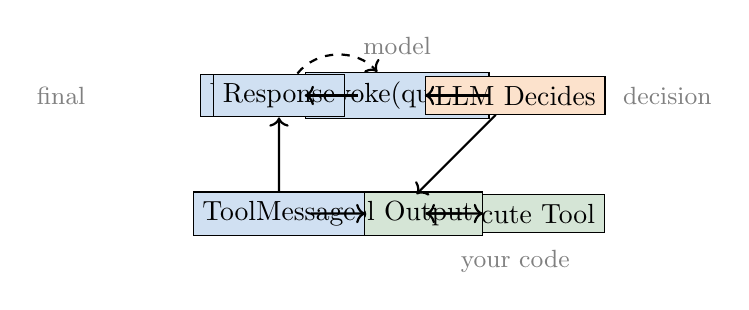
\begin{tikzpicture}[node distance=1.5cm, scale=0.85]
  % States
  \node[draw, rectangle, fill=lcblue!20] (user) {User Query};
  \node[draw, rectangle, fill=lcblue!20, right of=user] (invoke) {invoke(query)};
  \node[draw, rectangle, fill=lcorange!20, right of=invoke] (decide) {LLM Decides};
  \node[draw, rectangle, fill=lcorange!20, below of=invoke] (toolcalls) {tool\_calls};
  \node[draw, rectangle, fill=lcgreen!20, below of=decide] (execute) {Execute Tool};
  \node[draw, rectangle, fill=lcgreen!20, left of=execute] (result) {Tool Output};
  \node[draw, rectangle, fill=lcblue!20, left of=result] (toolmsg) {ToolMessage};
  \node[draw, rectangle, fill=lcblue!20, above of=toolmsg] (response) {Response};

  % Edges
  \draw[->, thick] (user) -- (invoke);
  \draw[->, thick] (invoke) -- (decide);
  \draw[->, thick] (decide) -- (toolcalls);
  \draw[->, thick] (toolcalls) -- (execute);
  \draw[->, thick] (execute) -- (result);
  \draw[->, thick] (result) -- (toolmsg);
  \draw[->, thick] (toolmsg) -- (response);
  \draw[->, thick, dashed] (response) to[bend left=50] (invoke);

  % Labels
  \node[above=0.1cm of invoke, anchor=south] {\small \color{gray}model};
  \node[right=0.1cm of decide, anchor=west] {\small \color{gray}decision};
  \node[below=0.1cm of execute, anchor=north] {\small \color{gray}your code};
  \node[left=1.5cm of response] {\small \color{gray}final};
\end{tikzpicture}
\end{center}
\vspace{-0.5cm}
Loop back for follow-up tool calls (agentic behavior).
\end{frame}

% ============================================================================
% SLIDE 22: Real-World Example: Simple Agent Loop
% ============================================================================
\begin{frame}[fragile]{Real-World Example: Simple Agent Loop}
\begin{codebox}[Tool-Based Agent Loop]
\begin{lstlisting}
from langchain.schema import HumanMessage, ToolMessage
from langchain_anthropic import ChatAnthropic
from langchain.tools import tool

@tool
def search(query: str) -> str:
    """Search documents."""
    return "Found information about " + query

model = ChatAnthropic().bind_tools([search])
messages = [HumanMessage("What is LangChain?")]

while True:
    response = model.invoke(messages)
    if not response.tool_calls:
        print("Final:", response.content)
        break

    # Execute each tool call
    for call in response.tool_calls:
        tool_result = search.invoke(
            call['args']
        )
        messages.append(
            ToolMessage(content=tool_result,
                       tool_call_id=call['id'])
        )
    messages.append(response)
\end{lstlisting}
\end{codebox}
\end{frame}

% ============================================================================
% SLIDE 23: Common Pitfall #1: Missing Descriptions
% ============================================================================
\begin{frame}[fragile]{Pitfall \#1: Missing or Vague Descriptions}
\begin{warningbox}[The Problem]
LLM doesn't know when to use your tool if description is missing or vague.
\end{warningbox}

\begin{codebox}[Bad: No Description]
\begin{lstlisting}
@tool
def foo(x: str) -> str:
    # No docstring!
    return "result"

# LLM: "I don't know what foo does"
\end{lstlisting}
\end{codebox}

\begin{codebox}[Good: Clear Description]
\begin{lstlisting}
@tool
def retrieve_document(doc_id: str) -> str:
    """Retrieve full document by unique ID.

    Use when user asks for specific documents
    by ID or when you need the full content.
    """
    return "Document content..."
\end{lstlisting}
\end{codebox}
\end{frame}

% ============================================================================
% SLIDE 24: Common Pitfall #2: Wrong Type Annotations
% ============================================================================
\begin{frame}[fragile]{Pitfall \#2: Missing or Wrong Type Annotations}
\begin{warningbox}[The Problem]
Without type hints, schema generation fails or becomes ambiguous.
\end{warningbox}

\begin{codebox}[Bad: No Type Hints]
\begin{lstlisting}
@tool
def process(data):
    # LLM: "What type is data? Can't call it"
    return data

# The function works but tool is unusable
\end{lstlisting}
\end{codebox}

\begin{codebox}[Good: Full Type Hints]
\begin{lstlisting}
from typing import List

@tool
def process(data: List[str]) -> str:
    """Process a list of strings."""
    return ", ".join(data)

# Now LLM knows: pass list of strings, get string
\end{lstlisting}
\end{codebox}
\end{frame}

% ============================================================================
% SLIDE 25: Common Pitfall #3: Not Returning ToolMessage
% ============================================================================
\begin{frame}[fragile]{Pitfall \#3: Forgetting ToolMessage in Chains}
\begin{warningbox}[The Problem]
If you don't wrap tool results in ToolMessage, the LLM can't properly track which result belongs to which tool.
\end{warningbox}

\begin{codebox}[Bad: No ToolMessage]
\begin{lstlisting}
response = model.invoke(user_query)
tool_result = my_tool.invoke(response.tool_calls[0]['args'])

# Directly appending raw result breaks context
messages.append(tool_result)  # WRONG!
\end{lstlisting}
\end{codebox}

\begin{codebox}[Good: Use ToolMessage]
\begin{lstlisting}
from langchain.schema import ToolMessage

tool_result = my_tool.invoke(call['args'])
messages.append(
    ToolMessage(
        content=tool_result,
        tool_call_id=call['id']
    )
)
\end{lstlisting}
\end{codebox}
\end{frame}

% ============================================================================
% SLIDE 26: Common Pitfall #4: Throwing Exceptions
% ============================================================================
\begin{frame}[fragile]{Pitfall \#4: Raising Exceptions Instead of Returning Errors}
\begin{warningbox}[The Problem]
Exceptions break the tool calling loop. Return errors as strings instead.
\end{warningbox}

\begin{codebox}[Bad: Raising Exceptions]
\begin{lstlisting}
@tool
def risky_operation(x: int) -> int:
    if x < 0:
        raise ValueError("x must be positive")
    return x * 2

# Tool call fails, loop breaks
\end{lstlisting}
\end{codebox}

\begin{codebox}[Good: Return Error Strings]
\begin{lstlisting}
@tool
def risky_operation(x: int) -> str:
    if x < 0:
        return "Error: x must be positive"
    return str(x * 2)

# LLM sees error and can retry/adjust
\end{lstlisting}
\end{codebox}
\end{frame}

% ============================================================================
% SLIDE 27: Common Pitfall #5: Tool with Side Effects
% ============================================================================
\begin{frame}[fragile]{Pitfall \#5: Tools with Unintended Side Effects}
\begin{warningbox}[The Problem]
Avoid tools that modify state unexpectedly. LLM might call them multiple times.
\end{warningbox}

\begin{codebox}[Bad: Side Effects]
\begin{lstlisting}
charge_count = 0

@tool
def charge_user(amount: float) -> str:
    global charge_count
    charge_count += 1
    # Actually charge the user
    # LLM calls twice = double charge!
    process_payment(amount)
    return "Charged"
\end{lstlisting}
\end{codebox}

\begin{codebox}[Good: Idempotent]
\begin{lstlisting}
@tool
def get_user_balance(user_id: str) -> str:
    """Read-only: Get balance."""
    return str(db.get_balance(user_id))

# Safe to call multiple times
\end{lstlisting}
\end{codebox}
\end{frame}

% ============================================================================
% SLIDE 28: Tool Composition with LCEL
% ============================================================================
\begin{frame}[fragile]{Tool Composition with LCEL}
\begin{codebox}[Compose Tools in Chains]
\begin{lstlisting}
from langchain_core.runnables import RunnablePassthrough
from langchain.tools import tool

@tool
def summarize(text: str) -> str:
    """Summarize text."""
    return text[:50] + "..."

@tool
def translate(text: str) -> str:
    """Translate to Spanish."""
    return "Translated: " + text

# Chain tools: pass output of one to next
chain = (
    RunnablePassthrough()
    | {"result": summarize}
    | lambda x: translate.invoke(x["result"])
)

output = chain.invoke("Long text here...")
\end{lstlisting}
\end{codebox}

Tools integrate naturally with LCEL chains.
\end{frame}

% ============================================================================
% SLIDE 29: Advanced: Tool Retry Logic
% ============================================================================
\begin{frame}[fragile]{Advanced: Retry Logic for Tools}
\begin{codebox}[Implement Tool Retries]
\begin{lstlisting}
from tenacity import retry, stop_after_attempt

@tool
@retry(stop=stop_after_attempt(3))
def flaky_api_call(query: str) -> str:
    """Call an API that might fail."""
    import random
    if random.random() < 0.5:
        raise Exception("API timeout")
    return f"Result for {query}"

# Decorator handles retries transparently
result = flaky_api_call.invoke({"query": "test"})
\end{lstlisting}
\end{codebox}

Combine LangChain tools with libraries like Tenacity for resilience.
\end{frame}

% ============================================================================
% SLIDE 30: Tool Monitoring and Logging
% ============================================================================
\begin{frame}[fragile]{Monitoring and Logging Tool Calls}
\begin{codebox}[Log Tool Invocations]
\begin{lstlisting}
import logging
from langchain.tools import tool

logger = logging.getLogger(__name__)

@tool
def logged_search(query: str) -> str:
    """Search with logging."""
    logger.info(f"Tool called: search, query={query}")
    result = "Results..."
    logger.info(f"Tool result: {result}")
    return result

# Or use LangChain callbacks (Section 10)
from langchain.callbacks import StdOutCallbackHandler
chain = model.bind_tools([logged_search])
chain.invoke(query, callbacks=[StdOutCallbackHandler()])
\end{lstlisting}
\end{codebox}

Track tool usage for debugging and analytics.
\end{frame}

% ============================================================================
% SLIDE 31: Tool Return Types and Serialization
% ============================================================================
\begin{frame}[fragile]{Return Types: What Tools Should Return}
\begin{codebox}[Return Types]
\begin{lstlisting}
from typing import Dict, List
import json

@tool
def get_structured_data(id: str) -> str:
    """Return structured data as JSON string."""
    data = {"id": id, "values": [1, 2, 3]}
    return json.dumps(data)

@tool
def get_simple_text(query: str) -> str:
    """Return plain text."""
    return f"Answer: {query}"

# Always return str for LLM consumption
# Use JSON strings for structured data
\end{lstlisting}
\end{codebox}

\begin{tipbox}[Best Practice]
Tools should return strings. Convert objects to JSON if needed.
\end{tipbox}
\end{frame}

% ============================================================================
% SLIDE 32: Tool Testing
% ============================================================================
\begin{frame}[fragile]{Testing Tools Independently}
\begin{codebox}[Unit Test Your Tools]
\begin{lstlisting}
from langchain.tools import tool
import pytest

@tool
def calculate_discount(price: float,
                       percent: int) -> str:
    """Apply discount to price."""
    if percent < 0 or percent > 100:
        return "Error: percent must be 0-100"
    result = price * (1 - percent / 100)
    return str(result)

def test_calculate_discount():
    result = calculate_discount.invoke({
        "price": 100,
        "percent": 10
    })
    assert result == "90.0"

    result = calculate_discount.invoke({
        "price": 100,
        "percent": 150
    })
    assert "Error" in result
\end{lstlisting}
\end{codebox}

Test tools like normal Python functions.
\end{frame}

% ============================================================================
% SLIDE 33: Best Practices Summary
% ============================================================================
\begin{frame}[fragile]{Tool Design Best Practices}
\begin{enumerate}
  \item \textbf{Clear descriptions}: Explain when to use the tool
  \item \textbf{Type annotations}: All parameters must have types
  \item \textbf{Good docstrings}: Include use cases in the docstring
  \item \textbf{Error handling}: Return errors as strings, not exceptions
  \item \textbf{Validation}: Use Pydantic for complex inputs
  \item \textbf{Idempotency}: Safe to call multiple times
  \item \textbf{Atomic}: One tool = one action
  \item \textbf{Testability}: Tools should be testable in isolation
  \item \textbf{Return strings}: LLMs consume text, use JSON for structured data
  \item \textbf{Performance}: Keep tools fast; use async for I/O
\end{enumerate}
\end{frame}

% ============================================================================
% SLIDE 34: Quick Reference / Cheat Sheet
% ============================================================================
\begin{frame}[fragile]{Quick Reference: Tools Cheat Sheet}
\begin{codebox}[The @tool Decorator Way (Quickest)]
\begin{lstlisting}
from langchain.tools import tool

@tool
def my_tool(arg1: str, arg2: int) -> str:
    """Description of what my_tool does."""
    return "result"

model = ChatAnthropic().bind_tools([my_tool])
response = model.invoke("Use my_tool")
\end{lstlisting}
\end{codebox}

\begin{codebox}[The StructuredTool Way (Complex)]
\begin{lstlisting}
from langchain.tools import StructuredTool
from pydantic import BaseModel

class Input(BaseModel):
    x: str

tool = StructuredTool.from_function(
    func=my_func, args_schema=Input
)
\end{lstlisting}
\end{codebox}
\end{frame}

% ============================================================================
% SLIDE 35: Self-Check Questions
% ============================================================================
\begin{frame}[fragile]{Self-Check: Do You Understand?}
\begin{enumerate}
  \item What's the difference between \texttt{@tool} and \texttt{StructuredTool}?
    \begin{itemize}\small
      \item \texttt{@tool}: Decorator for simple tools from functions (infers schema from type hints)
      \item \texttt{StructuredTool}: Explicit for complex tools with custom Pydantic schemas
    \end{itemize}

  \item What must you return after tool execution?
    \begin{itemize}\small
      \item \texttt{ToolMessage(content=result, tool\_call\_id=...)}
    \end{itemize}

  \item Why do tools need descriptions?
    \begin{itemize}\small
      \item LLM uses descriptions to decide when to call the tool
    \end{itemize}

  \item What happens if you raise an exception in a tool?
    \begin{itemize}\small
      \item The tool calling loop breaks; return errors as strings instead
    \end{itemize}
\end{enumerate}
\end{frame}

% ============================================================================
% SLIDE 36: Self-Check Questions (Continued)
% ============================================================================
\begin{frame}[fragile]{Self-Check: More Questions}
\begin{enumerate}
  \setcounter{enumi}{4}
  \item How do you attach tools to a model?
    \begin{itemize}\small
      \item Use \texttt{model.bind\_tools([tool1, tool2, ...])}, returns a new model with tools bound
    \end{itemize}

  \item What's the purpose of \texttt{tool\_choice="required"}?
    \begin{itemize}\small
      \item Forces the LLM to always call a tool (useful for agentic loops)
    \end{itemize}

  \item Can tools be called asynchronously?
    \begin{itemize}\small
      \item Yes, define them as \texttt{async def} and use \texttt{.ainvoke()}
    \end{itemize}

  \item What's an idempotent tool?
    \begin{itemize}\small
      \item One that returns the same result when called multiple times; safe for LLM retries
    \end{itemize}
\end{enumerate}
\end{frame}

% ============================================================================
% SLIDE 37: Key Takeaways
% ============================================================================
\begin{frame}[fragile]{Key Takeaways}
\begin{conceptbox}[Tools Enable Agency]
Tools are how LLMs move from passive text generation to active interaction with the world.
\end{conceptbox}

\vfill

\begin{tipbox}[Three Patterns]
\begin{itemize}
  \item \textbf{@tool}: Quick decorator for simple functions
  \item \textbf{StructuredTool}: Explicit schemas for complex tools
  \item \textbf{bind\_tools()}: Attach tools to models for calling
\end{itemize}
\end{tipbox}

\vfill

\begin{warningbox}[Remember]
LLM \textbf{decides} to call a tool, but \textbf{you} execute it and return ToolMessage with results.
\end{warningbox}
\end{frame}

% ============================================================================
% SLIDE 38: What's Next?
% ============================================================================
\begin{frame}[fragile]{What's Next?}
\begin{itemize}
  \item \textbf{Section 05: Agents}
    \begin{itemize}\small
      \item Agentic loops that autonomously use tools to solve problems
      \item Agent frameworks: ReAct, MRKL, conversational agents
    \end{itemize}

  \item \textbf{Section 11: LangGraph}
    \begin{itemize}\small
      \item Structured control flow for tool-using applications
      \item State machines and multi-step reasoning
    \end{itemize}

  \item \textbf{Section 10: Callbacks \& Monitoring}
    \begin{itemize}\small
      \item Track tool invocations, trace execution
    \end{itemize}
\end{itemize}

\vfill

Tools are the foundation for everything that follows!
\end{frame}

% ============================================================================
% SLIDE 39: References and Further Reading
% ============================================================================
\begin{frame}[fragile]{References \& Further Reading}
\begin{itemize}
  \item \textcolor{lcblue}{\textbf{Official LangChain Docs}}
    \begin{itemize}\small
      \item Tools: \texttt{https://python.langchain.com/docs/modules/tools/}
      \item Tool usage: \texttt{https://python.langchain.com/docs/modules/tools/tool\_use/}
    \end{itemize}

  \item \textcolor{lcblue}{\textbf{LangChain API Reference}}
    \begin{itemize}\small
      \item \texttt{langchain.tools}: Decorators and classes
      \item \texttt{langchain.schema}: Message types (ToolMessage)
    \end{itemize}

  \item \textcolor{lcblue}{\textbf{Agent Patterns}}
    \begin{itemize}\small
      \item ReAct paper: Yao et al., 2022
      \item Tool use with Claude: \texttt{https://docs.anthropic.com/}
    \end{itemize}
\end{itemize}

\docref{langchain.tools, langchain.schema.ToolMessage}
\end{frame}

% ============================================================================
% SLIDE 40: Conclusion
% ============================================================================
\begin{frame}[fragile]{Conclusion}
\begin{center}
\Large
\textbf{You now understand:}

\vfill

\normalsize
\begin{itemize}
  \item What tools are and why they matter
  \item How to create tools with decorators and schemas
  \item How to bind tools to models
  \item The tool calling flow and how to execute tools
  \item Common pitfalls and how to avoid them
  \item Advanced patterns: async, validation, monitoring
\end{itemize}

\vfill

\large
\textcolor{lcgreen}{\textbf{You're ready to build agentic applications!}}
\end{center}
\end{frame}

\end{document}
